% Created by tikzDevice version 0.7.0 on 2014-01-30 13:33:20
% !TEX encoding = UTF-8 Unicode
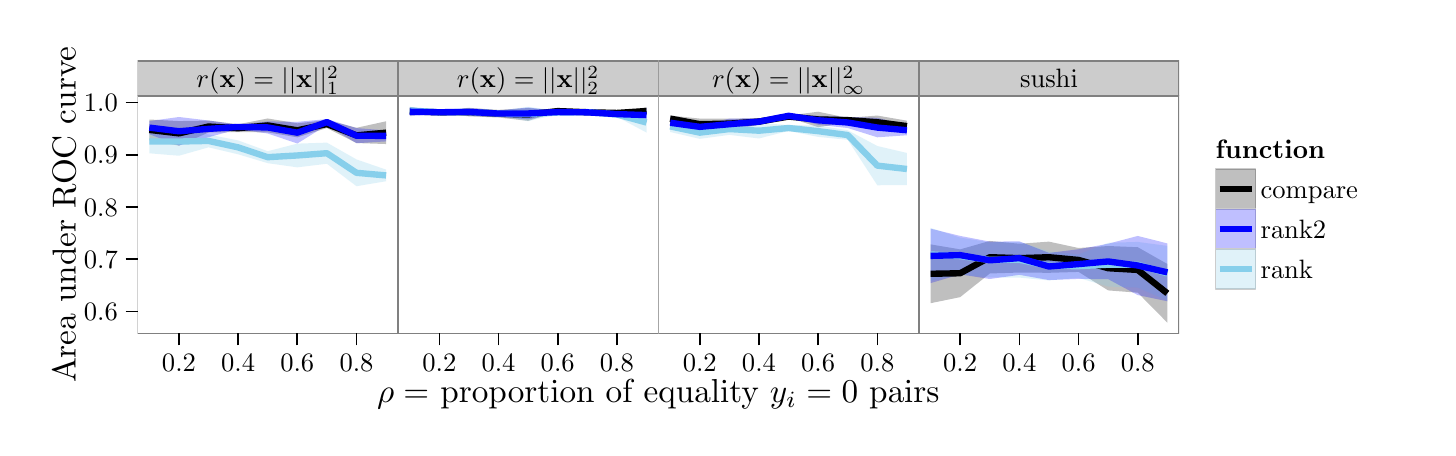
\begin{tikzpicture}[x=1pt,y=1pt]
\definecolor[named]{fillColor}{rgb}{1.00,1.00,1.00}
\path[use as bounding box,fill=fillColor,fill opacity=0.00] (0,0) rectangle (505.89,144.54);
\begin{scope}
\path[clip] (  0.00,  0.00) rectangle (505.89,144.54);
\definecolor[named]{drawColor}{rgb}{1.00,1.00,1.00}
\definecolor[named]{fillColor}{rgb}{1.00,1.00,1.00}

\path[draw=drawColor,line width= 0.6pt,line join=round,line cap=round,fill=fillColor] (  0.00,  0.00) rectangle (505.89,144.54);
\end{scope}
\begin{scope}
\path[clip] ( 39.69,119.86) rectangle (133.79,132.50);
\definecolor[named]{drawColor}{rgb}{0.50,0.50,0.50}
\definecolor[named]{fillColor}{rgb}{0.80,0.80,0.80}

\path[draw=drawColor,line width= 0.6pt,line join=round,line cap=round,fill=fillColor] ( 39.69,119.86) rectangle (133.79,132.50);
\definecolor[named]{drawColor}{rgb}{0.00,0.00,0.00}

\node[text=drawColor,anchor=base,inner sep=0pt, outer sep=0pt, scale=  0.96] at ( 86.74,122.87) {$r(\mathbf x) = ||\mathbf x||_1^2$};
\end{scope}
\begin{scope}
\path[clip] (133.79,119.86) rectangle (227.89,132.50);
\definecolor[named]{drawColor}{rgb}{0.50,0.50,0.50}
\definecolor[named]{fillColor}{rgb}{0.80,0.80,0.80}

\path[draw=drawColor,line width= 0.6pt,line join=round,line cap=round,fill=fillColor] (133.79,119.86) rectangle (227.89,132.50);
\definecolor[named]{drawColor}{rgb}{0.00,0.00,0.00}

\node[text=drawColor,anchor=base,inner sep=0pt, outer sep=0pt, scale=  0.96] at (180.84,122.87) {$r(\mathbf x) = ||\mathbf x||_2^2$};
\end{scope}
\begin{scope}
\path[clip] (227.89,119.86) rectangle (321.99,132.50);
\definecolor[named]{drawColor}{rgb}{0.50,0.50,0.50}
\definecolor[named]{fillColor}{rgb}{0.80,0.80,0.80}

\path[draw=drawColor,line width= 0.6pt,line join=round,line cap=round,fill=fillColor] (227.89,119.86) rectangle (321.99,132.50);
\definecolor[named]{drawColor}{rgb}{0.00,0.00,0.00}

\node[text=drawColor,anchor=base,inner sep=0pt, outer sep=0pt, scale=  0.96] at (274.94,122.87) {$r(\mathbf x) = ||\mathbf x||_\infty^2$};
\end{scope}
\begin{scope}
\path[clip] (321.99,119.86) rectangle (416.09,132.50);
\definecolor[named]{drawColor}{rgb}{0.50,0.50,0.50}
\definecolor[named]{fillColor}{rgb}{0.80,0.80,0.80}

\path[draw=drawColor,line width= 0.6pt,line join=round,line cap=round,fill=fillColor] (321.99,119.86) rectangle (416.09,132.50);
\definecolor[named]{drawColor}{rgb}{0.00,0.00,0.00}

\node[text=drawColor,anchor=base,inner sep=0pt, outer sep=0pt, scale=  0.96] at (369.04,122.87) {sushi};
\end{scope}
\begin{scope}
\path[clip] ( 39.69, 34.03) rectangle (133.79,119.86);
\definecolor[named]{fillColor}{rgb}{1.00,1.00,1.00}

\path[fill=fillColor] ( 39.69, 34.03) rectangle (133.79,119.86);
\definecolor[named]{fillColor}{rgb}{0.00,0.00,0.00}

\path[fill=fillColor,fill opacity=0.25] ( 43.96,111.35) --
	( 54.66,110.79) --
	( 65.35,110.96) --
	( 76.04,109.63) --
	( 86.74,111.72) --
	( 97.43,109.98) --
	(108.12,111.14) --
	(118.82,108.36) --
	(129.51,110.71) --
	(129.51,102.49) --
	(118.82,102.85) --
	(108.12,108.27) --
	( 97.43,104.92) --
	( 86.74,106.72) --
	( 76.04,106.80) --
	( 65.35,106.67) --
	( 54.66,101.91) --
	( 43.96,103.85) --
	cycle;
\definecolor[named]{fillColor}{rgb}{0.53,0.81,0.92}

\path[fill=fillColor,fill opacity=0.25] ( 43.96,107.63) --
	( 54.66,108.54) --
	( 65.35,105.92) --
	( 76.04,103.81) --
	( 86.74, 99.90) --
	( 97.43,102.64) --
	(108.12,103.00) --
	(118.82, 96.93) --
	(129.51, 93.25) --
	(129.51, 89.04) --
	(118.82, 87.25) --
	(108.12, 95.36) --
	( 97.43, 94.07) --
	( 86.74, 95.57) --
	( 76.04, 98.78) --
	( 65.35,101.30) --
	( 54.66, 98.26) --
	( 43.96, 99.15) --
	cycle;
\definecolor[named]{fillColor}{rgb}{0.00,0.00,1.00}

\path[fill=fillColor,fill opacity=0.25] ( 43.96,110.79) --
	( 54.66,112.26) --
	( 65.35,110.99) --
	( 76.04,109.46) --
	( 86.74,110.68) --
	( 97.43,110.50) --
	(108.12,111.50) --
	(118.82,108.24) --
	(129.51,107.42) --
	(129.51,103.44) --
	(118.82,102.79) --
	(108.12,109.33) --
	( 97.43,102.68) --
	( 86.74,106.30) --
	( 76.04,107.88) --
	( 65.35,104.95) --
	( 54.66,101.97) --
	( 43.96,106.05) --
	cycle;
\definecolor[named]{drawColor}{rgb}{0.00,0.00,0.00}

\path[draw=drawColor,line width= 2.3pt,line join=round] ( 43.96,107.60) --
	( 54.66,106.35) --
	( 65.35,108.82) --
	( 76.04,108.21) --
	( 86.74,109.22) --
	( 97.43,107.45) --
	(108.12,109.70) --
	(118.82,105.61) --
	(129.51,106.60);
\definecolor[named]{drawColor}{rgb}{0.53,0.81,0.92}

\path[draw=drawColor,line width= 2.3pt,line join=round] ( 43.96,103.39) --
	( 54.66,103.40) --
	( 65.35,103.61) --
	( 76.04,101.29) --
	( 86.74, 97.74) --
	( 97.43, 98.36) --
	(108.12, 99.18) --
	(118.82, 92.09) --
	(129.51, 91.15);
\definecolor[named]{drawColor}{rgb}{0.00,0.00,1.00}

\path[draw=drawColor,line width= 2.3pt,line join=round] ( 43.96,108.42) --
	( 54.66,107.11) --
	( 65.35,107.97) --
	( 76.04,108.67) --
	( 86.74,108.49) --
	( 97.43,106.59) --
	(108.12,110.42) --
	(118.82,105.51) --
	(129.51,105.43);
\definecolor[named]{drawColor}{rgb}{0.50,0.50,0.50}

\path[draw=drawColor,line width= 0.6pt,line join=round,line cap=round] ( 39.69, 34.03) rectangle (133.79,119.86);
\end{scope}
\begin{scope}
\path[clip] (133.79, 34.03) rectangle (227.89,119.86);
\definecolor[named]{fillColor}{rgb}{1.00,1.00,1.00}

\path[fill=fillColor] (133.79, 34.03) rectangle (227.89,119.86);
\definecolor[named]{fillColor}{rgb}{0.00,0.00,0.00}

\path[fill=fillColor,fill opacity=0.25] (138.07,115.91) --
	(148.76,114.22) --
	(159.45,115.53) --
	(170.15,114.84) --
	(180.84,115.49) --
	(191.53,114.63) --
	(202.23,114.82) --
	(212.92,113.99) --
	(223.61,115.77) --
	(223.61,113.07) --
	(212.92,113.45) --
	(202.23,113.15) --
	(191.53,114.15) --
	(180.84,110.86) --
	(170.15,112.08) --
	(159.45,112.51) --
	(148.76,113.63) --
	(138.07,112.75) --
	cycle;
\definecolor[named]{fillColor}{rgb}{0.53,0.81,0.92}

\path[fill=fillColor,fill opacity=0.25] (138.07,115.90) --
	(148.76,114.39) --
	(159.45,115.17) --
	(170.15,114.45) --
	(180.84,115.96) --
	(191.53,114.47) --
	(202.23,114.83) --
	(212.92,114.00) --
	(223.61,113.87) --
	(223.61,106.65) --
	(212.92,112.34) --
	(202.23,113.21) --
	(191.53,113.27) --
	(180.84,110.74) --
	(170.15,112.66) --
	(159.45,112.93) --
	(148.76,113.50) --
	(138.07,113.35) --
	cycle;
\definecolor[named]{fillColor}{rgb}{0.00,0.00,1.00}

\path[fill=fillColor,fill opacity=0.25] (138.07,115.84) --
	(148.76,114.43) --
	(159.45,115.60) --
	(170.15,114.63) --
	(180.84,115.70) --
	(191.53,114.37) --
	(202.23,114.86) --
	(212.92,113.74) --
	(223.61,115.53) --
	(223.61,110.37) --
	(212.92,112.87) --
	(202.23,113.02) --
	(191.53,113.74) --
	(180.84,111.39) --
	(170.15,112.38) --
	(159.45,112.59) --
	(148.76,113.54) --
	(138.07,112.54) --
	cycle;
\definecolor[named]{drawColor}{rgb}{0.00,0.00,0.00}

\path[draw=drawColor,line width= 2.3pt,line join=round] (138.07,114.33) --
	(148.76,113.93) --
	(159.45,114.02) --
	(170.15,113.46) --
	(180.84,113.17) --
	(191.53,114.39) --
	(202.23,113.98) --
	(212.92,113.72) --
	(223.61,114.42);
\definecolor[named]{drawColor}{rgb}{0.53,0.81,0.92}

\path[draw=drawColor,line width= 2.3pt,line join=round] (138.07,114.62) --
	(148.76,113.95) --
	(159.45,114.05) --
	(170.15,113.55) --
	(180.84,113.35) --
	(191.53,113.87) --
	(202.23,114.02) --
	(212.92,113.17) --
	(223.61,110.26);
\definecolor[named]{drawColor}{rgb}{0.00,0.00,1.00}

\path[draw=drawColor,line width= 2.3pt,line join=round] (138.07,114.19) --
	(148.76,113.98) --
	(159.45,114.09) --
	(170.15,113.51) --
	(180.84,113.54) --
	(191.53,114.05) --
	(202.23,113.94) --
	(212.92,113.31) --
	(223.61,112.95);
\definecolor[named]{drawColor}{rgb}{0.50,0.50,0.50}

\path[draw=drawColor,line width= 0.6pt,line join=round,line cap=round] (133.79, 34.03) rectangle (227.89,119.86);
\end{scope}
\begin{scope}
\path[clip] (227.89, 34.03) rectangle (321.99,119.86);
\definecolor[named]{fillColor}{rgb}{1.00,1.00,1.00}

\path[fill=fillColor] (227.89, 34.03) rectangle (321.99,119.86);
\definecolor[named]{fillColor}{rgb}{0.00,0.00,0.00}

\path[fill=fillColor,fill opacity=0.25] (232.17,112.78) --
	(242.86,111.69) --
	(253.55,111.64) --
	(264.25,111.82) --
	(274.94,112.76) --
	(285.63,114.17) --
	(296.33,111.95) --
	(307.02,112.78) --
	(317.72,110.93) --
	(317.72,107.02) --
	(307.02,107.96) --
	(296.33,110.29) --
	(285.63,108.59) --
	(274.94,112.05) --
	(264.25,109.39) --
	(253.55,108.09) --
	(242.86,107.64) --
	(232.17,110.59) --
	cycle;
\definecolor[named]{fillColor}{rgb}{0.53,0.81,0.92}

\path[fill=fillColor,fill opacity=0.25] (232.17,110.90) --
	(242.86,108.85) --
	(253.55,109.99) --
	(264.25,110.12) --
	(274.94,109.33) --
	(285.63,109.22) --
	(296.33,107.47) --
	(307.02,101.78) --
	(317.72, 99.27) --
	(317.72, 87.67) --
	(307.02, 87.59) --
	(296.33,104.01) --
	(285.63,105.07) --
	(274.94,107.23) --
	(264.25,104.50) --
	(253.55,105.80) --
	(242.86,104.37) --
	(232.17,106.84) --
	cycle;
\definecolor[named]{fillColor}{rgb}{0.00,0.00,1.00}

\path[fill=fillColor,fill opacity=0.25] (232.17,112.07) --
	(242.86,109.31) --
	(253.55,111.66) --
	(264.25,111.82) --
	(274.94,112.95) --
	(285.63,112.70) --
	(296.33,112.28) --
	(307.02,111.96) --
	(317.72,109.30) --
	(317.72,105.66) --
	(307.02,104.93) --
	(296.33,108.28) --
	(285.63,109.45) --
	(274.94,112.42) --
	(264.25,109.37) --
	(253.55,107.63) --
	(242.86,108.09) --
	(232.17,108.29) --
	cycle;
\definecolor[named]{drawColor}{rgb}{0.00,0.00,0.00}

\path[draw=drawColor,line width= 2.3pt,line join=round] (232.17,111.68) --
	(242.86,109.67) --
	(253.55,109.87) --
	(264.25,110.60) --
	(274.94,112.41) --
	(285.63,111.38) --
	(296.33,111.12) --
	(307.02,110.37) --
	(317.72,108.97);
\definecolor[named]{drawColor}{rgb}{0.53,0.81,0.92}

\path[draw=drawColor,line width= 2.3pt,line join=round] (232.17,108.87) --
	(242.86,106.61) --
	(253.55,107.90) --
	(264.25,107.31) --
	(274.94,108.28) --
	(285.63,107.15) --
	(296.33,105.74) --
	(307.02, 94.69) --
	(317.72, 93.47);
\definecolor[named]{drawColor}{rgb}{0.00,0.00,1.00}

\path[draw=drawColor,line width= 2.3pt,line join=round] (232.17,110.18) --
	(242.86,108.70) --
	(253.55,109.65) --
	(264.25,110.59) --
	(274.94,112.69) --
	(285.63,111.08) --
	(296.33,110.28) --
	(307.02,108.44) --
	(317.72,107.48);
\definecolor[named]{drawColor}{rgb}{0.50,0.50,0.50}

\path[draw=drawColor,line width= 0.6pt,line join=round,line cap=round] (227.89, 34.03) rectangle (321.99,119.86);
\end{scope}
\begin{scope}
\path[clip] (321.99, 34.03) rectangle (416.09,119.86);
\definecolor[named]{fillColor}{rgb}{1.00,1.00,1.00}

\path[fill=fillColor] (321.99, 34.03) rectangle (416.09,119.86);
\definecolor[named]{fillColor}{rgb}{0.00,0.00,0.00}

\path[fill=fillColor,fill opacity=0.25] (326.27, 66.23) --
	(336.96, 64.43) --
	(347.66, 67.47) --
	(358.35, 66.46) --
	(369.04, 67.22) --
	(379.74, 64.92) --
	(390.43, 65.64) --
	(401.12, 65.21) --
	(411.82, 59.15) --
	(411.82, 37.94) --
	(401.12, 48.78) --
	(390.43, 49.60) --
	(379.74, 56.28) --
	(369.04, 55.96) --
	(358.35, 56.05) --
	(347.66, 55.72) --
	(336.96, 47.17) --
	(326.27, 44.98) --
	cycle;
\definecolor[named]{fillColor}{rgb}{0.53,0.81,0.92}

\path[fill=fillColor,fill opacity=0.25] (326.27, 72.19) --
	(336.96, 68.69) --
	(347.66, 66.98) --
	(358.35, 67.14) --
	(369.04, 63.73) --
	(379.74, 62.63) --
	(390.43, 66.81) --
	(401.12, 67.12) --
	(411.82, 65.69) --
	(411.82, 45.84) --
	(401.12, 50.63) --
	(390.43, 50.98) --
	(379.74, 54.12) --
	(369.04, 53.21) --
	(358.35, 54.23) --
	(347.66, 54.29) --
	(336.96, 55.29) --
	(326.27, 52.98) --
	cycle;
\definecolor[named]{fillColor}{rgb}{0.00,0.00,1.00}

\path[fill=fillColor,fill opacity=0.25] (326.27, 71.91) --
	(336.96, 69.29) --
	(347.66, 67.24) --
	(358.35, 67.31) --
	(369.04, 63.15) --
	(379.74, 64.47) --
	(390.43, 66.46) --
	(401.12, 69.28) --
	(411.82, 66.58) --
	(411.82, 45.67) --
	(401.12, 47.92) --
	(390.43, 53.67) --
	(379.74, 53.76) --
	(369.04, 53.34) --
	(358.35, 55.23) --
	(347.66, 53.72) --
	(336.96, 55.40) --
	(326.27, 52.24) --
	cycle;
\definecolor[named]{drawColor}{rgb}{0.00,0.00,0.00}

\path[draw=drawColor,line width= 2.3pt,line join=round] (326.27, 55.61) --
	(336.96, 55.80) --
	(347.66, 61.60) --
	(358.35, 61.26) --
	(369.04, 61.59) --
	(379.74, 60.60) --
	(390.43, 57.62) --
	(401.12, 57.00) --
	(411.82, 48.54);
\definecolor[named]{drawColor}{rgb}{0.53,0.81,0.92}

\path[draw=drawColor,line width= 2.3pt,line join=round] (326.27, 62.59) --
	(336.96, 61.99) --
	(347.66, 60.63) --
	(358.35, 60.69) --
	(369.04, 58.47) --
	(379.74, 58.37) --
	(390.43, 58.89) --
	(401.12, 58.88) --
	(411.82, 55.76);
\definecolor[named]{drawColor}{rgb}{0.00,0.00,1.00}

\path[draw=drawColor,line width= 2.3pt,line join=round] (326.27, 62.08) --
	(336.96, 62.34) --
	(347.66, 60.48) --
	(358.35, 61.27) --
	(369.04, 58.24) --
	(379.74, 59.11) --
	(390.43, 60.06) --
	(401.12, 58.60) --
	(411.82, 56.12);
\definecolor[named]{drawColor}{rgb}{0.50,0.50,0.50}

\path[draw=drawColor,line width= 0.6pt,line join=round,line cap=round] (321.99, 34.03) rectangle (416.09,119.86);
\end{scope}
\begin{scope}
\path[clip] (  0.00,  0.00) rectangle (505.89,144.54);
\definecolor[named]{drawColor}{rgb}{0.00,0.00,0.00}

\node[text=drawColor,anchor=base east,inner sep=0pt, outer sep=0pt, scale=  0.96] at ( 32.57, 38.70) {0.6};

\node[text=drawColor,anchor=base east,inner sep=0pt, outer sep=0pt, scale=  0.96] at ( 32.57, 57.56) {0.7};

\node[text=drawColor,anchor=base east,inner sep=0pt, outer sep=0pt, scale=  0.96] at ( 32.57, 76.43) {0.8};

\node[text=drawColor,anchor=base east,inner sep=0pt, outer sep=0pt, scale=  0.96] at ( 32.57, 95.30) {0.9};

\node[text=drawColor,anchor=base east,inner sep=0pt, outer sep=0pt, scale=  0.96] at ( 32.57,114.16) {1.0};
\end{scope}
\begin{scope}
\path[clip] (  0.00,  0.00) rectangle (505.89,144.54);
\definecolor[named]{drawColor}{rgb}{0.00,0.00,0.00}

\path[draw=drawColor,line width= 0.6pt,line join=round] ( 35.42, 42.00) --
	( 39.69, 42.00);

\path[draw=drawColor,line width= 0.6pt,line join=round] ( 35.42, 60.87) --
	( 39.69, 60.87);

\path[draw=drawColor,line width= 0.6pt,line join=round] ( 35.42, 79.74) --
	( 39.69, 79.74);

\path[draw=drawColor,line width= 0.6pt,line join=round] ( 35.42, 98.60) --
	( 39.69, 98.60);

\path[draw=drawColor,line width= 0.6pt,line join=round] ( 35.42,117.47) --
	( 39.69,117.47);
\end{scope}
\begin{scope}
\path[clip] (  0.00,  0.00) rectangle (505.89,144.54);
\definecolor[named]{drawColor}{rgb}{0.00,0.00,0.00}

\path[draw=drawColor,line width= 0.6pt,line join=round] ( 54.66, 29.77) --
	( 54.66, 34.03);

\path[draw=drawColor,line width= 0.6pt,line join=round] ( 76.04, 29.77) --
	( 76.04, 34.03);

\path[draw=drawColor,line width= 0.6pt,line join=round] ( 97.43, 29.77) --
	( 97.43, 34.03);

\path[draw=drawColor,line width= 0.6pt,line join=round] (118.82, 29.77) --
	(118.82, 34.03);
\end{scope}
\begin{scope}
\path[clip] (  0.00,  0.00) rectangle (505.89,144.54);
\definecolor[named]{drawColor}{rgb}{0.00,0.00,0.00}

\node[text=drawColor,anchor=base,inner sep=0pt, outer sep=0pt, scale=  0.96] at ( 54.66, 20.31) {0.2};

\node[text=drawColor,anchor=base,inner sep=0pt, outer sep=0pt, scale=  0.96] at ( 76.04, 20.31) {0.4};

\node[text=drawColor,anchor=base,inner sep=0pt, outer sep=0pt, scale=  0.96] at ( 97.43, 20.31) {0.6};

\node[text=drawColor,anchor=base,inner sep=0pt, outer sep=0pt, scale=  0.96] at (118.82, 20.31) {0.8};
\end{scope}
\begin{scope}
\path[clip] (  0.00,  0.00) rectangle (505.89,144.54);
\definecolor[named]{drawColor}{rgb}{0.00,0.00,0.00}

\path[draw=drawColor,line width= 0.6pt,line join=round] (148.76, 29.77) --
	(148.76, 34.03);

\path[draw=drawColor,line width= 0.6pt,line join=round] (170.15, 29.77) --
	(170.15, 34.03);

\path[draw=drawColor,line width= 0.6pt,line join=round] (191.53, 29.77) --
	(191.53, 34.03);

\path[draw=drawColor,line width= 0.6pt,line join=round] (212.92, 29.77) --
	(212.92, 34.03);
\end{scope}
\begin{scope}
\path[clip] (  0.00,  0.00) rectangle (505.89,144.54);
\definecolor[named]{drawColor}{rgb}{0.00,0.00,0.00}

\node[text=drawColor,anchor=base,inner sep=0pt, outer sep=0pt, scale=  0.96] at (148.76, 20.31) {0.2};

\node[text=drawColor,anchor=base,inner sep=0pt, outer sep=0pt, scale=  0.96] at (170.15, 20.31) {0.4};

\node[text=drawColor,anchor=base,inner sep=0pt, outer sep=0pt, scale=  0.96] at (191.53, 20.31) {0.6};

\node[text=drawColor,anchor=base,inner sep=0pt, outer sep=0pt, scale=  0.96] at (212.92, 20.31) {0.8};
\end{scope}
\begin{scope}
\path[clip] (  0.00,  0.00) rectangle (505.89,144.54);
\definecolor[named]{drawColor}{rgb}{0.00,0.00,0.00}

\path[draw=drawColor,line width= 0.6pt,line join=round] (242.86, 29.77) --
	(242.86, 34.03);

\path[draw=drawColor,line width= 0.6pt,line join=round] (264.25, 29.77) --
	(264.25, 34.03);

\path[draw=drawColor,line width= 0.6pt,line join=round] (285.63, 29.77) --
	(285.63, 34.03);

\path[draw=drawColor,line width= 0.6pt,line join=round] (307.02, 29.77) --
	(307.02, 34.03);
\end{scope}
\begin{scope}
\path[clip] (  0.00,  0.00) rectangle (505.89,144.54);
\definecolor[named]{drawColor}{rgb}{0.00,0.00,0.00}

\node[text=drawColor,anchor=base,inner sep=0pt, outer sep=0pt, scale=  0.96] at (242.86, 20.31) {0.2};

\node[text=drawColor,anchor=base,inner sep=0pt, outer sep=0pt, scale=  0.96] at (264.25, 20.31) {0.4};

\node[text=drawColor,anchor=base,inner sep=0pt, outer sep=0pt, scale=  0.96] at (285.63, 20.31) {0.6};

\node[text=drawColor,anchor=base,inner sep=0pt, outer sep=0pt, scale=  0.96] at (307.02, 20.31) {0.8};
\end{scope}
\begin{scope}
\path[clip] (  0.00,  0.00) rectangle (505.89,144.54);
\definecolor[named]{drawColor}{rgb}{0.00,0.00,0.00}

\path[draw=drawColor,line width= 0.6pt,line join=round] (336.96, 29.77) --
	(336.96, 34.03);

\path[draw=drawColor,line width= 0.6pt,line join=round] (358.35, 29.77) --
	(358.35, 34.03);

\path[draw=drawColor,line width= 0.6pt,line join=round] (379.74, 29.77) --
	(379.74, 34.03);

\path[draw=drawColor,line width= 0.6pt,line join=round] (401.12, 29.77) --
	(401.12, 34.03);
\end{scope}
\begin{scope}
\path[clip] (  0.00,  0.00) rectangle (505.89,144.54);
\definecolor[named]{drawColor}{rgb}{0.00,0.00,0.00}

\node[text=drawColor,anchor=base,inner sep=0pt, outer sep=0pt, scale=  0.96] at (336.96, 20.31) {0.2};

\node[text=drawColor,anchor=base,inner sep=0pt, outer sep=0pt, scale=  0.96] at (358.35, 20.31) {0.4};

\node[text=drawColor,anchor=base,inner sep=0pt, outer sep=0pt, scale=  0.96] at (379.74, 20.31) {0.6};

\node[text=drawColor,anchor=base,inner sep=0pt, outer sep=0pt, scale=  0.96] at (401.12, 20.31) {0.8};
\end{scope}
\begin{scope}
\path[clip] (  0.00,  0.00) rectangle (505.89,144.54);
\definecolor[named]{drawColor}{rgb}{0.00,0.00,0.00}

\node[text=drawColor,anchor=base,inner sep=0pt, outer sep=0pt, scale=  1.20] at (227.89,  9.03) {$\rho =$ proportion of equality $y_i=0$ pairs};
\end{scope}
\begin{scope}
\path[clip] (  0.00,  0.00) rectangle (505.89,144.54);
\definecolor[named]{drawColor}{rgb}{0.00,0.00,0.00}

\node[text=drawColor,rotate= 90.00,anchor=base,inner sep=0pt, outer sep=0pt, scale=  1.20] at ( 17.30, 76.95) {Area under ROC curve};
\end{scope}
\begin{scope}
\path[clip] (  0.00,  0.00) rectangle (505.89,144.54);
\definecolor[named]{fillColor}{rgb}{1.00,1.00,1.00}

\path[fill=fillColor] (424.96, 45.88) rectangle (484.98,108.02);
\end{scope}
\begin{scope}
\path[clip] (  0.00,  0.00) rectangle (505.89,144.54);
\definecolor[named]{drawColor}{rgb}{0.00,0.00,0.00}

\node[text=drawColor,anchor=base west,inner sep=0pt, outer sep=0pt, scale=  0.96] at (429.23, 97.12) {\bfseries function};
\end{scope}
\begin{scope}
\path[clip] (  0.00,  0.00) rectangle (505.89,144.54);
\definecolor[named]{drawColor}{rgb}{0.80,0.80,0.80}
\definecolor[named]{fillColor}{rgb}{1.00,1.00,1.00}

\path[draw=drawColor,line width= 0.6pt,line join=round,line cap=round,fill=fillColor] (429.23, 79.06) rectangle (443.68, 93.51);
\end{scope}
\begin{scope}
\path[clip] (  0.00,  0.00) rectangle (505.89,144.54);
\definecolor[named]{fillColor}{rgb}{0.00,0.00,0.00}

\path[fill=fillColor,fill opacity=0.25] (429.23, 79.06) rectangle (443.68, 93.51);

\path[] (429.23, 79.06) --
	(443.68, 93.51);
\end{scope}
\begin{scope}
\path[clip] (  0.00,  0.00) rectangle (505.89,144.54);
\definecolor[named]{drawColor}{rgb}{0.00,0.00,0.00}

\path[draw=drawColor,line width= 2.3pt,line join=round] (430.68, 86.28) -- (442.24, 86.28);
\end{scope}
\begin{scope}
\path[clip] (  0.00,  0.00) rectangle (505.89,144.54);
\definecolor[named]{drawColor}{rgb}{0.80,0.80,0.80}
\definecolor[named]{fillColor}{rgb}{1.00,1.00,1.00}

\path[draw=drawColor,line width= 0.6pt,line join=round,line cap=round,fill=fillColor] (429.23, 64.60) rectangle (443.68, 79.06);
\end{scope}
\begin{scope}
\path[clip] (  0.00,  0.00) rectangle (505.89,144.54);
\definecolor[named]{fillColor}{rgb}{0.00,0.00,1.00}

\path[fill=fillColor,fill opacity=0.25] (429.23, 64.60) rectangle (443.68, 79.06);

\path[] (429.23, 64.60) --
	(443.68, 79.06);
\end{scope}
\begin{scope}
\path[clip] (  0.00,  0.00) rectangle (505.89,144.54);
\definecolor[named]{drawColor}{rgb}{0.00,0.00,1.00}

\path[draw=drawColor,line width= 2.3pt,line join=round] (430.68, 71.83) -- (442.24, 71.83);
\end{scope}
\begin{scope}
\path[clip] (  0.00,  0.00) rectangle (505.89,144.54);
\definecolor[named]{drawColor}{rgb}{0.80,0.80,0.80}
\definecolor[named]{fillColor}{rgb}{1.00,1.00,1.00}

\path[draw=drawColor,line width= 0.6pt,line join=round,line cap=round,fill=fillColor] (429.23, 50.15) rectangle (443.68, 64.60);
\end{scope}
\begin{scope}
\path[clip] (  0.00,  0.00) rectangle (505.89,144.54);
\definecolor[named]{fillColor}{rgb}{0.53,0.81,0.92}

\path[fill=fillColor,fill opacity=0.25] (429.23, 50.15) rectangle (443.68, 64.60);

\path[] (429.23, 50.15) --
	(443.68, 64.60);
\end{scope}
\begin{scope}
\path[clip] (  0.00,  0.00) rectangle (505.89,144.54);
\definecolor[named]{drawColor}{rgb}{0.53,0.81,0.92}

\path[draw=drawColor,line width= 2.3pt,line join=round] (430.68, 57.37) -- (442.24, 57.37);
\end{scope}
\begin{scope}
\path[clip] (  0.00,  0.00) rectangle (505.89,144.54);
\definecolor[named]{drawColor}{rgb}{0.00,0.00,0.00}

\node[text=drawColor,anchor=base west,inner sep=0pt, outer sep=0pt, scale=  0.96] at (445.49, 82.98) {compare};
\end{scope}
\begin{scope}
\path[clip] (  0.00,  0.00) rectangle (505.89,144.54);
\definecolor[named]{drawColor}{rgb}{0.00,0.00,0.00}

\node[text=drawColor,anchor=base west,inner sep=0pt, outer sep=0pt, scale=  0.96] at (445.49, 68.52) {rank2};
\end{scope}
\begin{scope}
\path[clip] (  0.00,  0.00) rectangle (505.89,144.54);
\definecolor[named]{drawColor}{rgb}{0.00,0.00,0.00}

\node[text=drawColor,anchor=base west,inner sep=0pt, outer sep=0pt, scale=  0.96] at (445.49, 54.07) {rank};
\end{scope}
\end{tikzpicture}
